% Text removed from main.tex in v21 step 1 (2026-11-08); to be moved into supplement.tex where useful. Not compiled.
\begin{figure*}[t]
\centering
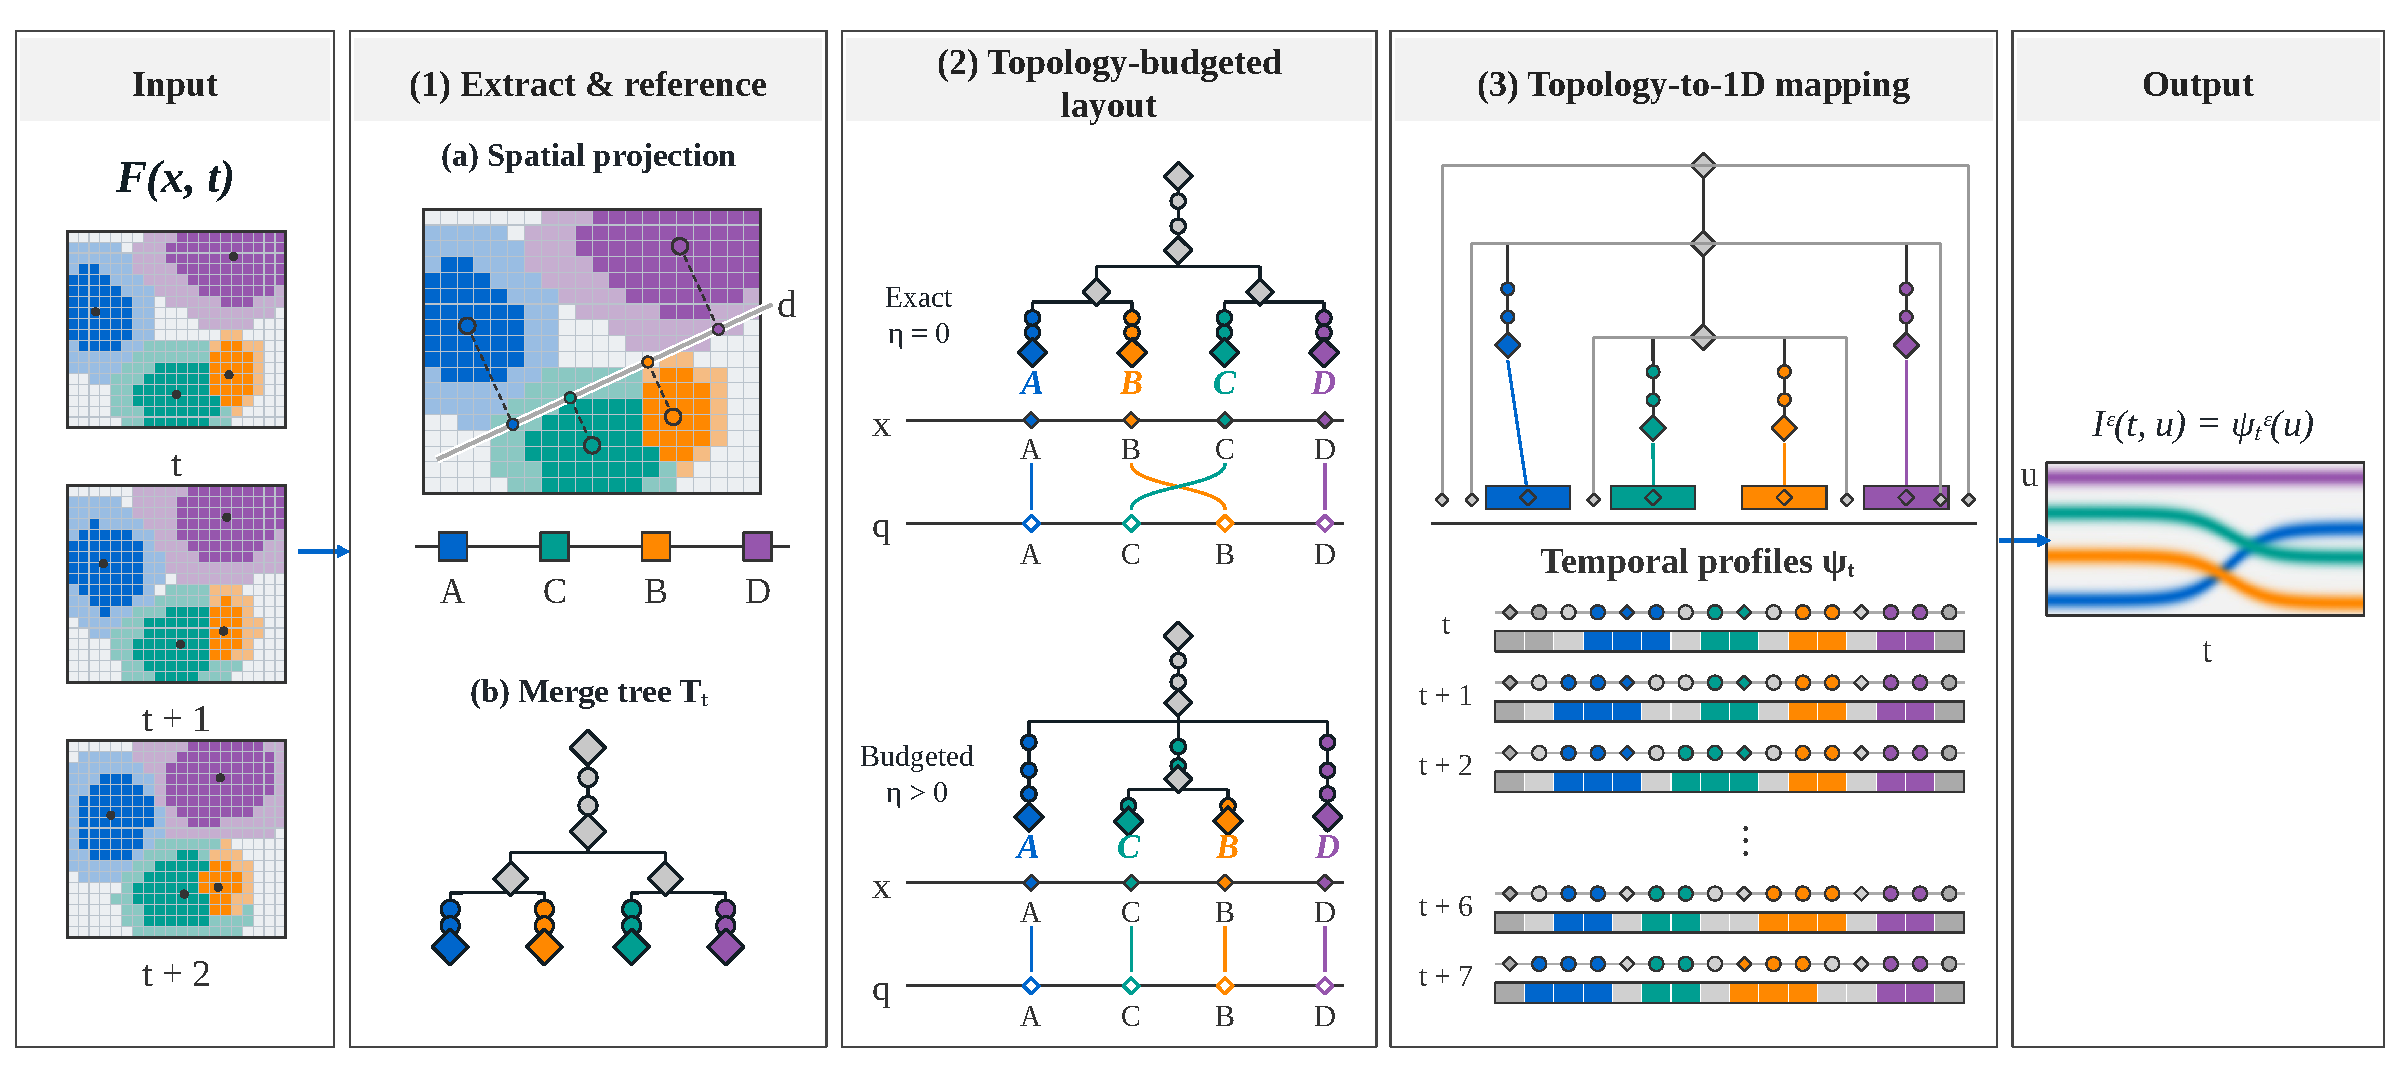
\includegraphics[width=\textwidth]{figures/anchor_framework.pdf}
\caption{AnchorMTM construction. (1) Extract augmented merge trees and match leaf supports, then estimate one fixed spatial reference from matched extremum motion. (2) Refine candidate leaf orders, admit those satisfying the merge-error allowance, and select by fixed-order displacement and NROE. (3) Optimize anchors within nonoverlapping intervals under a displacement cap, using valid matched history. (4) Reconstruct scalar profiles with barrier correction and assemble the temporal map. Diagrams are schematic; the map is an existing qualitative Storms output at $\varepsilon=10\%$. Order search is heuristic, and continuous feasibility and rendered errors are checked separately.}
\label{fig:framework}
\end{figure*}





\section{Background}\label{sec:background}
\subsection{Augmented Merge Trees and Feature Supports}
For a sampled 2D or 3D field $f_t:D\to\mathbb{R}$, the merge tree $T_t$ records sublevel-set connectivity: minima create components and saddles join them as the threshold increases. Negating the field gives the split-tree convention. Critical points are supernodes connected by superarcs; augmentation associates regular vertices with these arcs~\cite{Koepp:2023:TMTM,STMTM:2026,Tierny:2018:TTK}. Extraction and simplification precede layout.

A leaf represents an extremum at spatial location $p_i^t$. Its feature support $S_i^t$ consists of that extremum and the regular samples on its incident leaf arc, excluding the parent critical sample. It is not the full component or the complete subtree above that arc. For cross-frame overlap, these supports are sets of stable spatial sample IDs: the same ID must denote the same spatial sample across frames. Fixed-grid inputs preserve this identity through consistent sample indexing. Internal arcs retain further regular samples for scalar filling. Write $\mathcal{D}_t(v)$ for the descendant leaf labels of a node $v$, and $h_t(v)$ for its scalar level. The lowest common ancestor determines the merge-height matrix:
\begin{equation}\label{eq:merge}
 V_{ij}^t=h_t(\lca(i,j)),\quad i\ne j;\qquad
 V_{ii}^t=f_t(p_i^t).
\end{equation}
Equal-level merge events form one multifurcation; arbitrary binary refinements do not add strict constraints. All subsequent guarantees refer to the supplied, possibly simplified tree.

\subsection{One-Dimensional Merge-Tree Profiles}
A 1D merge-tree profile represents extrema at anchors in a selected leaf order. Regular vertices on leaf arcs supply scalar context within leaf intervals; internal arcs and paths to the LCA supply the intervening gaps~\cite{Koepp:2023:TMTM,STMTM:2026}. In join convention, extrema become profile minima, and the largest profile value between two anchors gives their displayed merge level. Exact preservation requires each strict subtree to occupy a contiguous leaf block. Arranging these profiles along time yields a static temporal map. This profile model provides the basis for the spatial anchoring formulation below.




\section{AnchorMTM}\label{sec:method}
Figure~\ref{fig:framework} summarizes the construction. AnchorMTM connects a shared spatial reference to the displayed leaf anchors. We construct the reference and formulate the layout, describe the construction, and then explain its unavoidable position costs through certified bounds. Analysis uses join convention; split-tree scalar signs are restored after reconstruction.

\subsection{Spatial Reference and Problem Formulation}\label{sec:reference}
\paragraph{Cross-frame Leaf Correspondence.}
We track merge-tree leaf extrema $p_i^t$ using their leaf-arc supports $S_i^t$. On a shared fixed grid, overlap-based preprocessing~\cite{STMTM:2026} counts common spatial samples:
\begin{equation}\label{eq:overlap}
 O_{ij}^t=|S_i^t\cap S_j^{t+1}|.
\end{equation}
Hungarian assignment maximizes total intersection count over one-to-one pairs, discarding zero-overlap pairs. The assigned links define the identity states described below.

\emph{Continuation} inherits a Track ID; \emph{birth/death} starts an unmatched current identity or ends an unmatched previous track. For \emph{non-bijective correspondence}, including potential one-to-many, many-to-one and ambiguous relations, only the assigned one-to-one links are retained. These identity states neither identify physical split/merge events nor form a branching lineage. For a current leaf $i$, $\mu_t(i)$ denotes its valid predecessor. The layout receives precomputed tracks aligned to leaf rows; upstream support and confidence conventions are detailed in Supplementary Material.

% Previous correspondence figure temporarily removed; source preserved in figures/source/open_mechanisms_20261106/.

These correspondences, computed before any topology-budget sweep, provide the motion samples for Spatial Anchoring, which distinguishes a reference target $q_i^t$ from the display anchor $x_i^t$. Only valid consecutive-frame matches contribute displacements; failed matches or interrupted tracks contribute no sample for that step. By default, one unit direction $a^*\in\mathbb{R}^d$, $d\in\{2,3\}$, is estimated offline from all matched consecutive-frame extremum displacements:
\begin{equation}\label{eq:autodirection}
\begin{aligned}
 \Delta p_i^t&=p_i^t-p_{\mu_t(i)}^{t-1},\\
 S&=\sum_{t,i\;\mathrm{matched}}\Delta p_i^t(\Delta p_i^t)^\top,\\
 a^*&\in\arg\max_{\|a\|=1}a^\top Sa.
\end{aligned}
\end{equation}
The leading eigenvector maximizes squared projected motion, not feature count or topological compatibility. The same calculation serves 2D and 3D; it is performed once for the whole sequence. Its sign makes total signed projected motion nonnegative; for near-zero signed motion, the largest-magnitude component is made positive. With negligible motion energy, the longest domain axis is used (first axis on a tie). Repeated leading eigenvalues leave the maximizing direction nonunique; the reported eigengap indicates this ambiguity. A supplied physical direction may replace $a^*$ without changing the layout. Overlap matching may miss fast-moving features or those with changing or weakly overlapping supports, affecting the displacement sample and hence the estimated direction.



\begin{figure}[t]
\centering
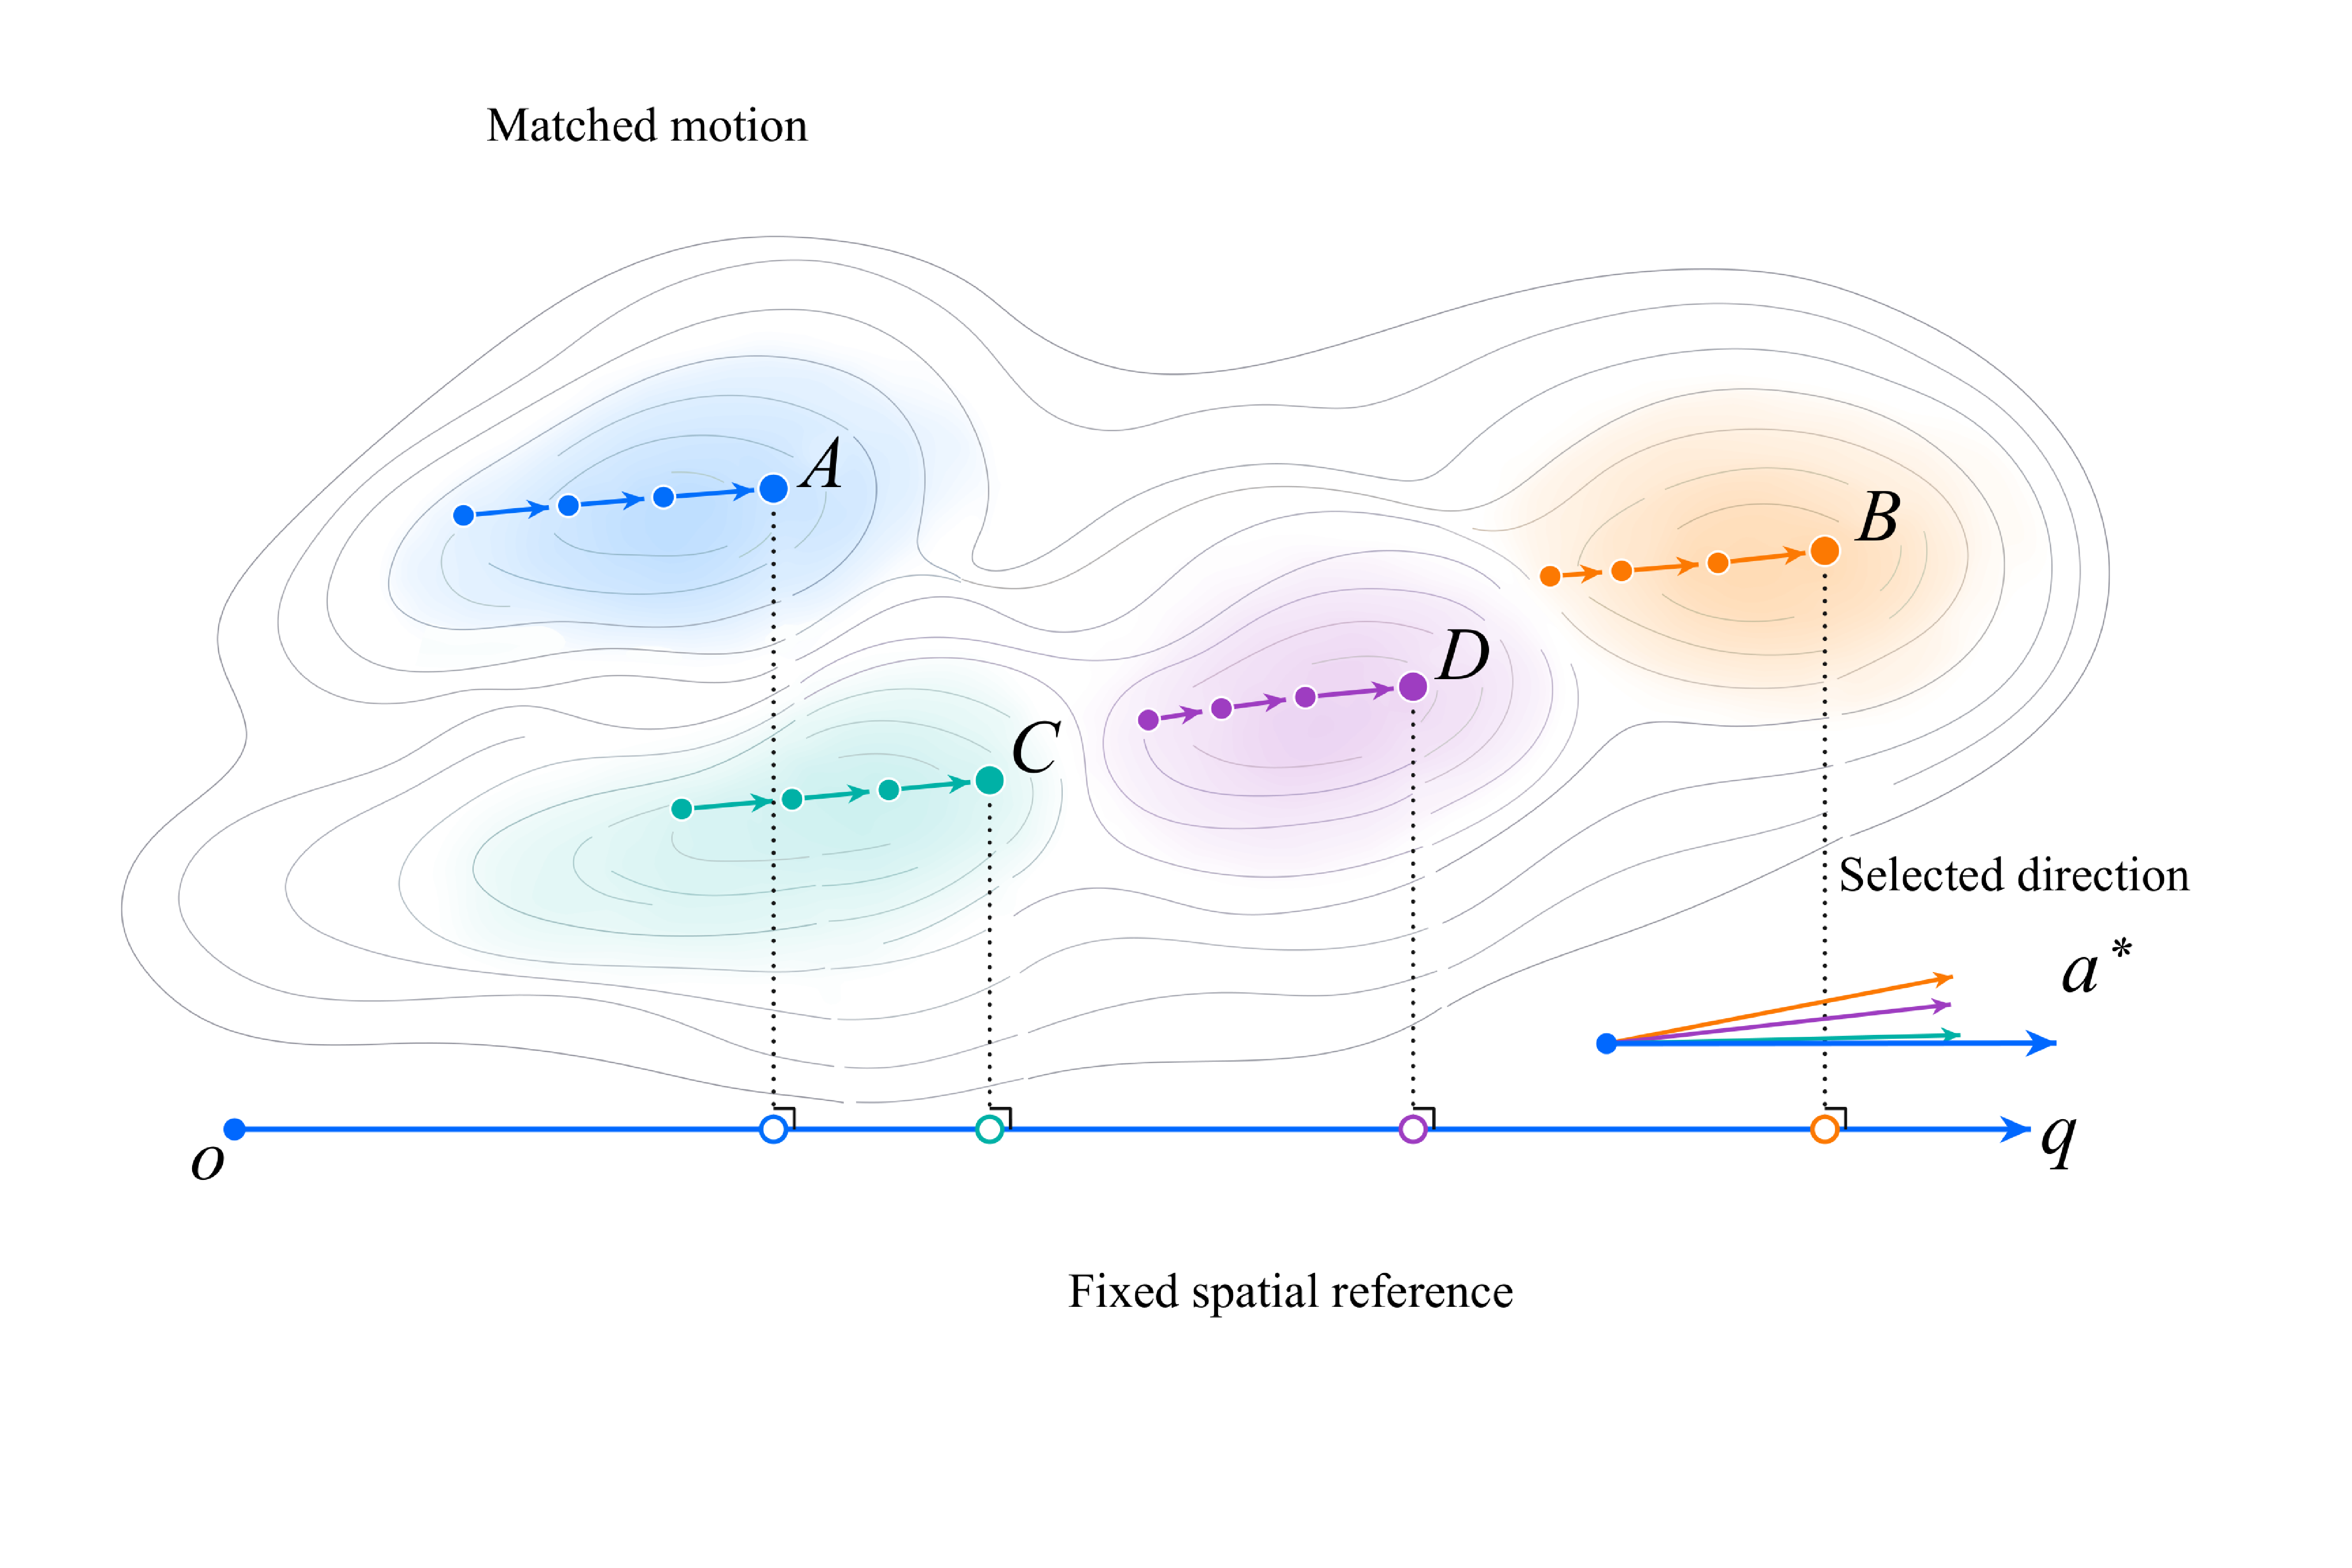
\includegraphics[width=0.85\columnwidth]{figures/anchor_direction_open.pdf}
\caption{Motion-derived spatial reference. Matched extremum displacements define one direction $a^*$ for the sequence; extrema project onto the parallel reference axis $q$ from a common origin $o$. Tracks, contours and projection positions are schematic.}
\label{fig:direction-open}
\end{figure}
Figure~\ref{fig:direction-open} illustrates the shared reference. For the selected direction, the minimum and span of the projected domain bounding-box corners define a common origin $o$ and extent $L>0$. The reference is
\begin{equation}\label{eq:reference}
 q_i^t=\langle a^*,p_i^t\rangle-o\in[0,L].
\end{equation}
Direction, origin and scale remain fixed across frames and all budgets for the same prepared sequence. Distinct extrema can share projected coordinates while retaining separate identities. Anchoring minimizes constrained deviation rather than requiring $x_i^t=q_i^t$.

Relative geometry uses distances $d_{ij}^t$ between leaf-support centroids. These differ from extremum references because a changing support can move its centroid while the extremum stays fixed. The automatic-reference adapter supplies extrema explicitly; the low-level solver also accepts precomputed references and otherwise defaults to centroid projection. Widths $W_i^t=s\,m_i^t$ convert positive support measures with a fixed scale $s$, without per-frame normalization.

Figure~\ref{fig:projection_conflict} contrasts the spatial target order with a tree-consistent order. In this four-minimum example, projected order $A,C,D,B$ separates $A$ and $B$ by the $C,D$ subtree, violating the required contiguity of $\{A,B\}$; exact topology therefore cannot realize all four targets without displacement.



With correspondence and the reference fixed, a frame comprises a leaf order, extremum anchors, and a scalar profile:
\begin{equation}\label{eq:mapframe}
 M_t=(\pi_t,x_t,\psi_t),\qquad\psi_t:[0,L]\to\mathbb{R}.
\end{equation}
We seek reference-aligned positions and motion while approximating relative geometry and controlling displayed topology. The interval-layout set $\mathcal{L}(\pi)$ requires intervals of widths $W_i$ centered at $z_i$ to lie inside the canvas, remain disjoint with gap at least $g\ge0$, and contain anchors satisfying $|x_i-z_i|\le\rho W_i/2$, $0\le\rho\le1$. Infeasible total widths and gaps are reported rather than rescaled.

Actual displacement is $|x_i-q_i|$, normalized by $L$ when reported. To distinguish order conflict from finite-width placement, define
\begin{equation}\label{eq:nroe}
 \nroe(\pi)=\frac{1}{2L}\max_{j\le k}
                      [q_{\pi(j)}-q_{\pi(k)}]^+.
\end{equation}
This is the smallest worst displacement of a nondecreasing point placement, divided by $L$; it ignores widths. For finite intervals, the exact fixed-order cost is
\begin{equation}\label{eq:tau}
 \tau(\pi)=\min_{(x,z)\in\mathcal{L}(\pi)}\|x-q\|_\infty.
\end{equation}
The minimum is attained whenever the layout set is nonempty. It is evaluated exactly from the fixed-order packing constraints, equivalently through a minimax linear program.

For distinct labels, let $V_{ij}^{\psi}$ be the maximum profile value between their anchors, with $V_{ii}^{\psi}=\psi(x_i)$. We require
\begin{equation}\label{eq:dtop}
\begin{aligned}
 \dtop(\psi_t,T_t)&=\max_{i,j}|V_{ij}^{\psi_t}-V_{ij}^t|\le\eta,\\
 \eta&=(\varepsilon_0+\varepsilon)\Delta_F.
\end{aligned}
\end{equation}
Here $\Delta_F>0$ is the sequence-wide scalar range, $\varepsilon_0$ is a fixed numerical allowance, and $\varepsilon\ge0$ is the sole primary user control. The implementation defaults to $\varepsilon_0=10^{-7}$. NMLE reports the achieved normalized error $\dtop/\Delta_F$. Exact topology means zero labelled error on the declared tree. A nonzero tie allowance is accounted for in $\eta$.

All remaining settings belong to a fixed configuration $\Theta_0$: position slack $\beta_0$, the four objective weights, width scale, gap, anchor slack and output resolution. For a prepared sequence, the default interface is $M_t^\varepsilon=\operatorname{AnchorMTM}(T_t,q_t,W_t,V_t,\mu_t;\varepsilon,\Theta_0)$. Advanced settings may be supplied once, but only $\varepsilon$ varies in a budget sweep. Supplementary Material specifies the fixed scale rules and implementation tolerances.

For canonical cophenetic merge-tree representations whose fixed labels cover every leaf and whose induced matrices include the diagonal, $\dtop$ equals the unnormalized labelled interleaving distance~\cite{Munch:2019:LINF,Gasparovic:2024:IID}. Under these conditions, $d_B\le d_I\le\dtop$~\cite{Morozov:2013:IDMT}. Unlabelled extrema introduced by rendering must be checked before applying this interpretation to the whole displayed tree.

\begin{figure}[t]
\centering
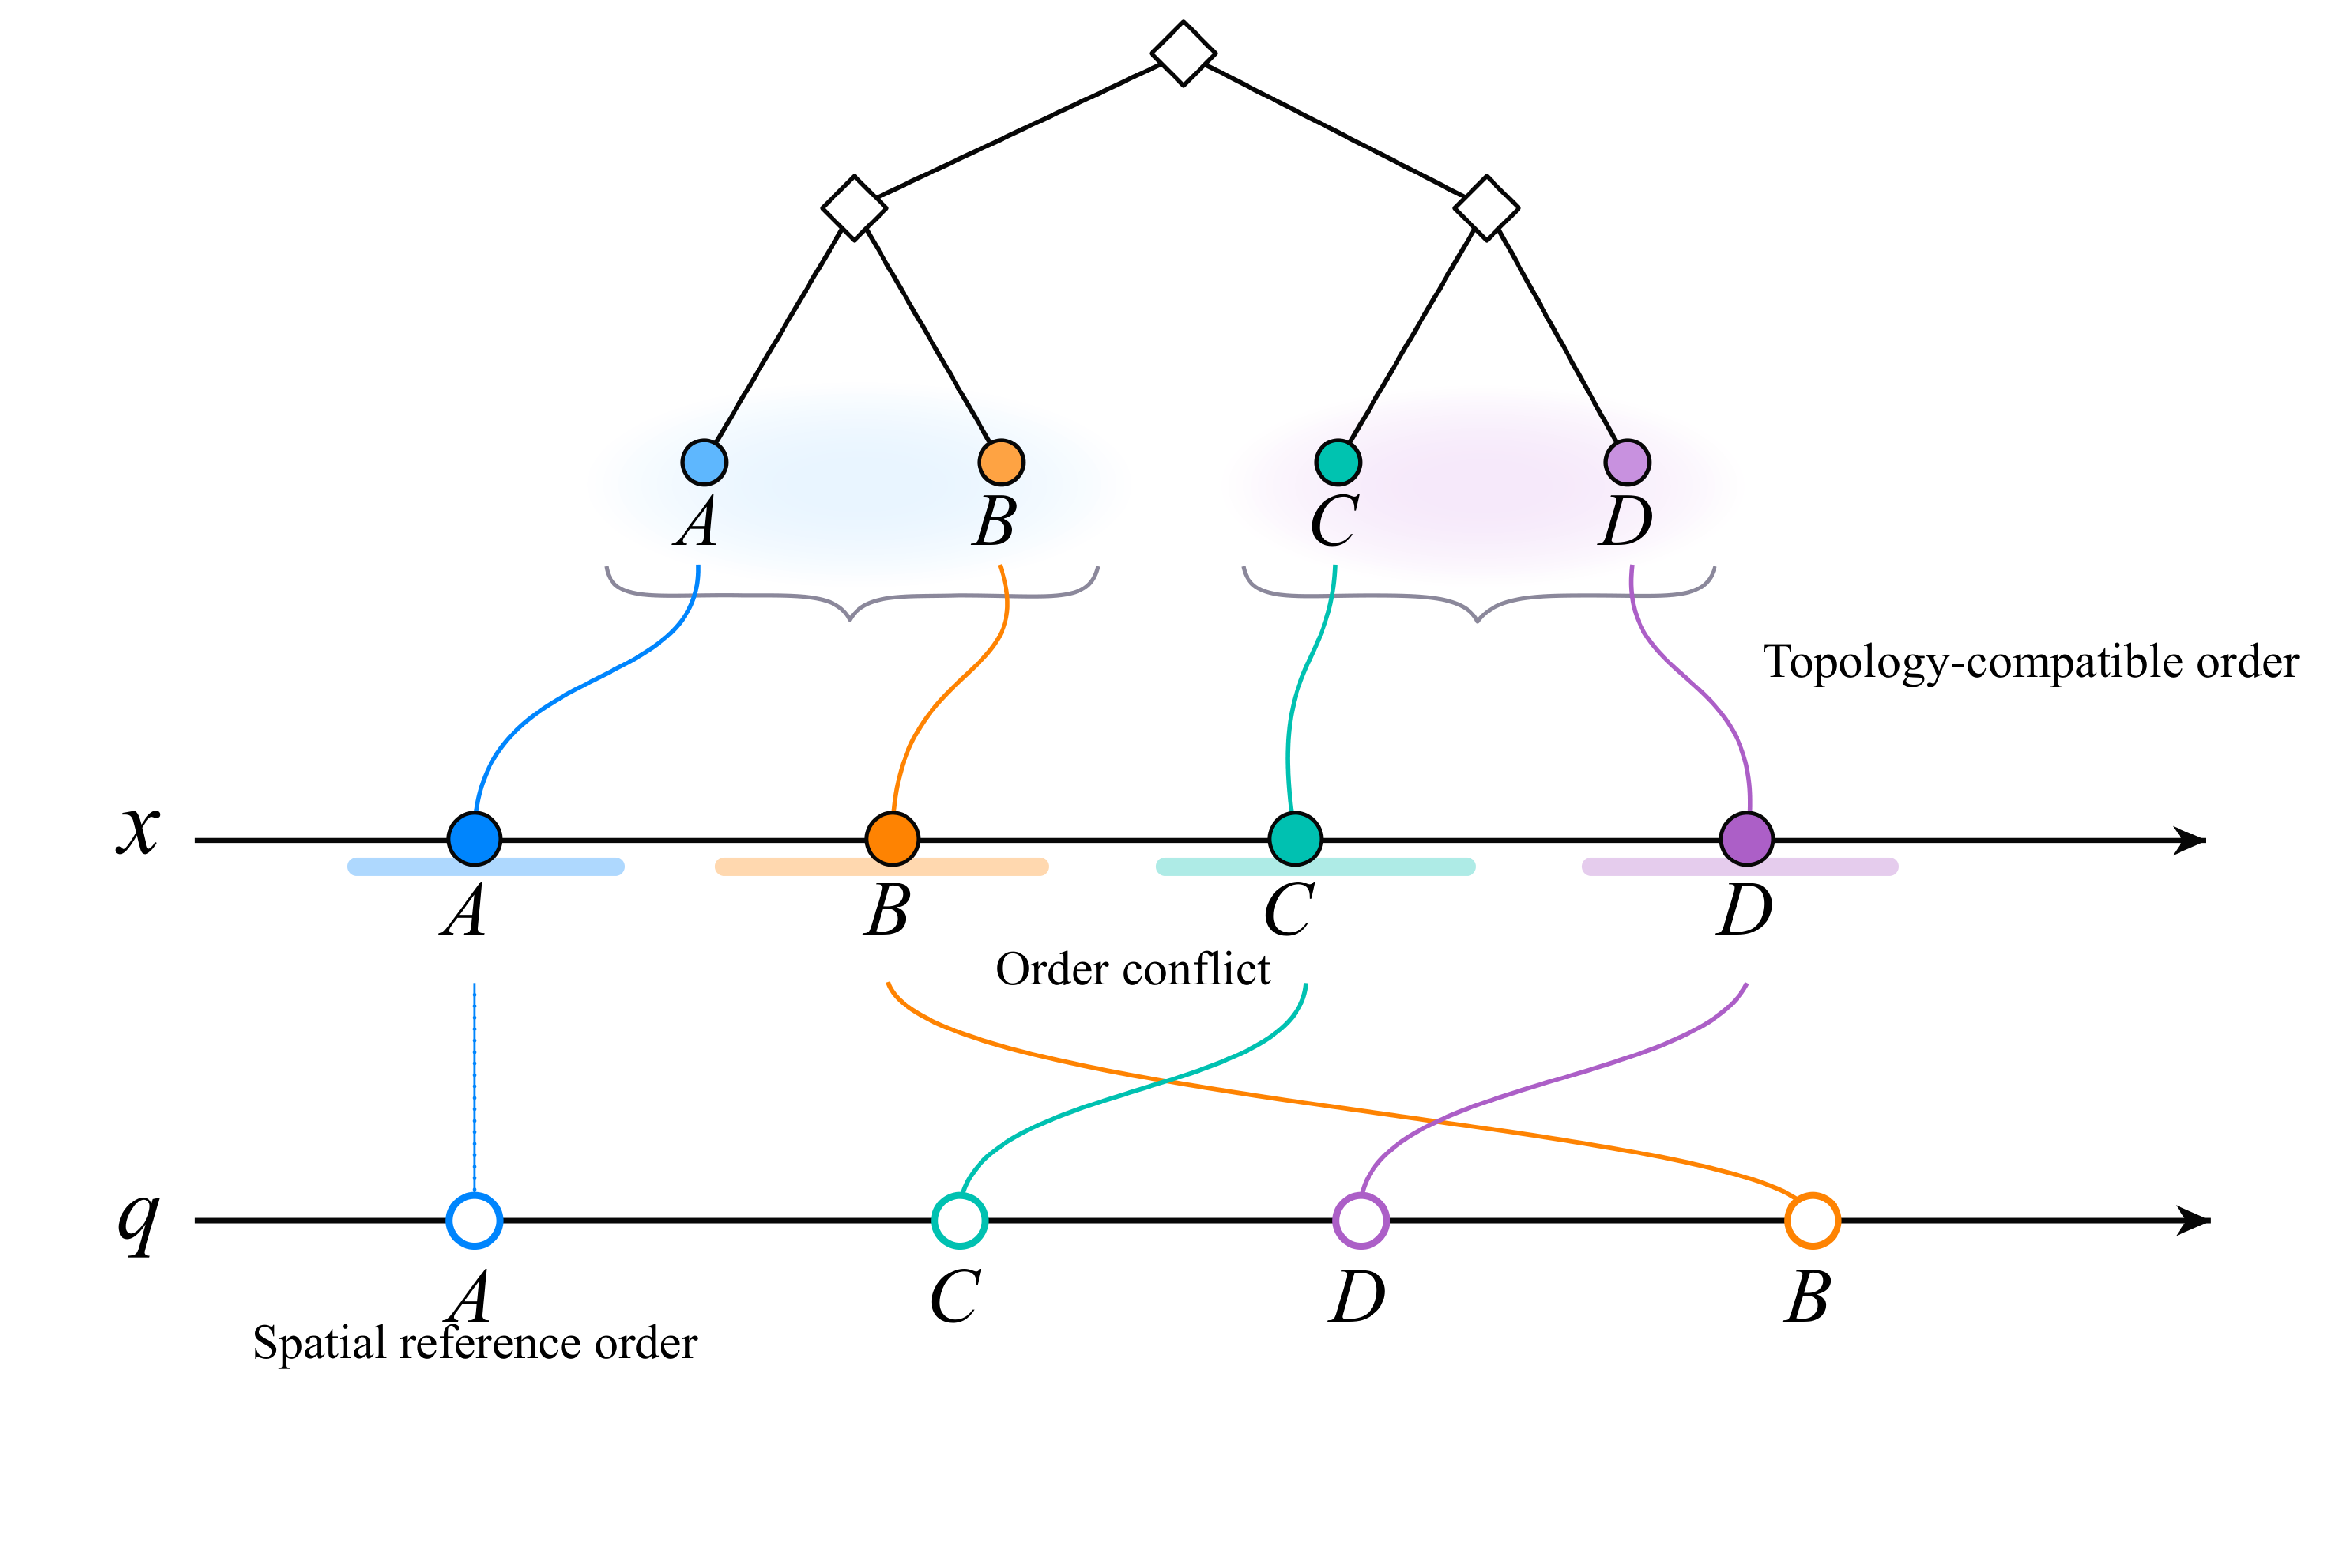
\includegraphics[width=\columnwidth]{figures/anchor_conflict_open.pdf}
\caption{Reference--topology conflict. The tree requires contiguous $A,B$ and $C,D$ blocks. Its displayed anchors $x$ follow a compatible order, whereas the fixed spatial targets $q$ occur as $A,C,D,B$. Colored links indicate the displacement needed to reconcile these orders. Widths and positions are schematic.}
\label{fig:projection_conflict}
\end{figure}
\subsection{Spatially Anchored Layout Construction}\label{sec:construction}
With features and their reference fixed, construction chooses an order by the lexicographic objective
\begin{equation}\label{eq:orderobjective}
\begin{aligned}
 \pi_t^\varepsilon&\in\underset{\pi\in\mathcal{C}_t(\varepsilon)}{\arg\min}
                    \bigl(\tau_t(\pi),\nroe_t(\pi)\bigr),\\
 &\hspace{1em}\mathrm{s.t.}\quad\delta_t^*(\pi)\le\eta(\varepsilon).
\end{aligned}
\end{equation}
The finite candidate pool contains the original strict-topology order, midpoint initializations, and orders visited during width-aware refinement of threshold and selective flattenings. Every candidate is evaluated against the same source merge matrix. Selection minimizes $\tau$ first and NROE second; it is not a global optimum over all permutations. Algorithm~\ref{alg:construction} separates this discrete selection from fixed-order placement.

\begin{algorithm}[htbp]
\caption{Single-Control AnchorMTM}\label{alg:construction}
\KwData{2D/3D field sequence and grid; $\varepsilon\ge0$; fixed configuration $\Theta_0$.}
\KwResult{Temporal map $I^\varepsilon$, error records, or a failure report.}
Extract augmented trees, leaf supports and extrema; match supports and assign Track IDs\;
Estimate one direction and fixed references $q_t$; reuse this preprocessing across budgets\;
$\eta\leftarrow(\varepsilon_0+\varepsilon)\Delta_F$\;
\For{each time step $t$ in temporal order}{
 Report and stop if widths and gaps exceed the fixed canvas\;
 $\mathcal{C}_t\leftarrow\operatorname{GenerateAndRefine}(T_t,q_t,W_t,V_t,\eta)$; retain strict-topology candidates\;
 Evaluate $\tau(\pi)$, $\nroe(\pi)$ and $\delta^*(\pi)$ for candidates\;
 $\mathcal{F}_t\leftarrow\{\pi\in\mathcal{C}_t:\delta^*(\pi)\le\eta\}$\;
 \lIf{$\mathcal{F}_t=\varnothing$}{report no feasible candidate and stop}
 Select $\pi_t^\varepsilon$ from $\mathcal{F}_t$ by $(\tau,\nroe)$\;
 Compute optimal merge barriers for $\pi_t^\varepsilon$\;
 Solve the four-term QP only for $\pi_t^\varepsilon$, with cap $\tau(\pi_t^\varepsilon)+\beta_0$ and valid matched history\;
 Reconstruct the profile by leaf/LCA filling and barrier correction\;
 Record candidate counts, continuous and rendered errors, motion and failures; append profile to $I^\varepsilon$\;
}
\KwReturn{$I^\varepsilon$ and diagnostic records}\;
\end{algorithm}

\subsubsection{Topology-Budgeted Leaf Ordering}
\emph{Exact Mode} sets $\varepsilon=0$, leaving only the numerical allowance $\eta=\varepsilon_0\Delta_F$, which merges saddles tied to within $\varepsilon_0\Delta_F$; strict exact topology is $\eta=0$. \emph{Budgeted Mode} permits $\varepsilon>0$. Both modes share the same interval model and placement objective.

Candidate generation includes the exact tree, threshold flattenings, and a conflict-driven selective flattening. Midpoint orders initialize these structures. Width-aware block insertion refines the four best initial structures, together with the exact tree, while retaining the point-model budget order as a candidate. Moves improve the lexicographic score consisting of $\tau$ and a squared packing-residual term, and must pass $\delta^*(\pi)\le\eta$. Visited initial and trial orders are retained in the deduplicated pool, including the strict-tree initialization and retained point candidate. Final budget filtering and lexicographic selection use the exact fixed-order costs; refinement does not certify a global optimum over permutations. 

Figure~\ref{fig:selective_relaxation} illustrates the additional ordering freedom created by a selective flattening. Removing the $A$--$B$ sibling constraint admits the order $A,C,D,B$ while retaining the $C$--$D$ subtree. This structural proposal still requires evaluation against the original merge matrix and the prescribed error budget.



Helpers inherit the current geometry and layout parameters. Comparisons use the implementation's numerical tolerances. The guards report capacity failure or an empty admitted set; no widths, gaps or canvas scales are silently changed. The exact-tree structure is always retained among refinement seeds, and its child-block moves preserve strict topology in the exact model. Its presence does not guarantee successful numerical placement or raster reconstruction; capacity, input and solver failures remain possible. An empty admitted set is never selected from. Invalid input and numerical solver failures propagate as errors, separately from mathematical infeasibility. First-frame and unmatched history contributes no temporal target.

\subsubsection{Optimal Merge Barriers and Topological Feasibility}
For a fixed order, a pair's displayed merge is the largest intervening barrier. Set $C_k=\min_{i\le k<j}V_{\pi(i)\pi(j)}$ and $F_k=\max(V_{\pi(k)\pi(k)},V_{\pi(k+1)\pi(k+1)})$ for gap $k$.
\begin{proposition}[Optimal barriers]\label{prop:barriers}
With fixed extremum values in the continuous non-strict model, the smallest labelled merge error is
\begin{equation}\label{eq:delta}
\begin{split}
 \delta^*(\pi)=\max\bigg\{&0,\max_k(F_k-C_k),\\
 &\frac12\max_{i<j}\left(V_{\pi(i)\pi(j)}-
                         \max_{i\le k<j}C_k\right)\bigg\},
\end{split}
\end{equation}
and barriers $b_k=C_k+\delta^*(\pi)$ attain it.
\end{proposition}
Error $\delta$ requires $F_k\le b_k\le C_k+\delta$. Choosing the largest admissible barriers satisfies every pair's lower merge requirement exactly when $\delta\ge\delta^*$. Thus the order meets the merge-level allowance in this continuous model exactly when $\delta^*(\pi)\le\eta$. This fixed-order test supports candidate search without making it globally optimal. Strict-extremum clearance and raster effects are checked separately.

\subsubsection{Spatially Anchored Spatiotemporal Placement}
Once the order is fixed, the core terms are $E_R$, mean squared deviation from the fixed reference, and $E_M$, mean squared error in matched projected motion. The auxiliary term $E_G$ approximates support-centroid distances through ordered anchor separations; $E_C$ regularizes anchor offsets from interval centers. All four terms and their nonnegative weights are retained:
\begin{equation}\label{eq:qp}
\begin{aligned}
 \min_{x_t,z_t}\quad&\lambda_R E_R+\lambda_G E_G+\lambda_M E_M+\lambda_C E_C\\
 \mathrm{s.t.}\quad&(x_t,z_t)\in\mathcal{L}(\pi_t),\\
 &\|x_t-q_t\|_\infty\le\tau(\pi_t)+\beta_0.
\end{aligned}
\end{equation}
For each valid match, set $\Delta q_i^t=q_i^t-q_{\mu_t(i)}^{t-1}$ and use the previous display anchor plus this reference displacement as the temporal target:
\begin{equation}\label{eq:temporal_target}
 \hat x_i^t=x_{\mu_t(i)}^{t-1}+(q_i^t-q_{\mu_t(i)}^{t-1}).
\end{equation}
Thus $E_M$ follows projected motion while favoring continuity of $x-q$. First-frame, newly born and otherwise unmatched leaves have no previous-frame motion penalty. Each term is averaged over its features, ordered pairs or valid matches; the current automatic-reference adapter uses unit confidence for valid matches. Supplementary Material distinguishes this default from legacy confidence-weighted paths.

Only $\varepsilon$ changes the topology allowance $\eta(\varepsilon)$. The fixed slack $\beta_0\ge0$ bounds additional position deviation after ordering. The cap is feasible because $\tau(\pi_t)$ is attained; the QP receives only the selected order and cannot replace it by one with a lower quadratic objective. It bounds continuous displacement while geometry and temporal objectives select a compromise within that cap. The fixed-order problem is convex; sequential processing does not imply a joint sequence optimum or exact preservation of every projected motion.

\subsubsection{Profile Reconstruction and Output Diagnostics}
Reconstruction inherits the leaf-arc sampling and LCA-path filling of the merge tree map pipeline~\cite{Koepp:2023:TMTM,STMTM:2026}. Original extrema remain at their anchors; regular samples provide scalar context within intervals and gaps. Optimal-barrier correction then clips each inter-anchor interior to $b_k$ and raises an existing peak if necessary. This separate correction is required for relaxed orders; inherited LCA filling alone does not enforce the minimax barriers.

A common direction, origin, extent, and pixel conversion are used for all frames. The profiles form the final temporal map,
\begin{equation}\label{eq:map}
 I^\varepsilon(t,u)=\psi_t^\varepsilon(u),\qquad 0\le u\le L.
\end{equation}
There is no per-frame recentering. Resampling does not retain every source sample, and corrected interior values need not remain in the original scalar range. Strict-extremum clearance and raster rounding can change the achieved error. Full-tree interpretation additionally requires checking label coverage. A recorded profile is therefore not unconditionally certified by $\delta^*\le\eta$. Records distinguish the requested budget, position certificates, attained $\tau$, continuous $\delta^*$, and actual rendered errors. 

\begin{figure}[t]
\centering
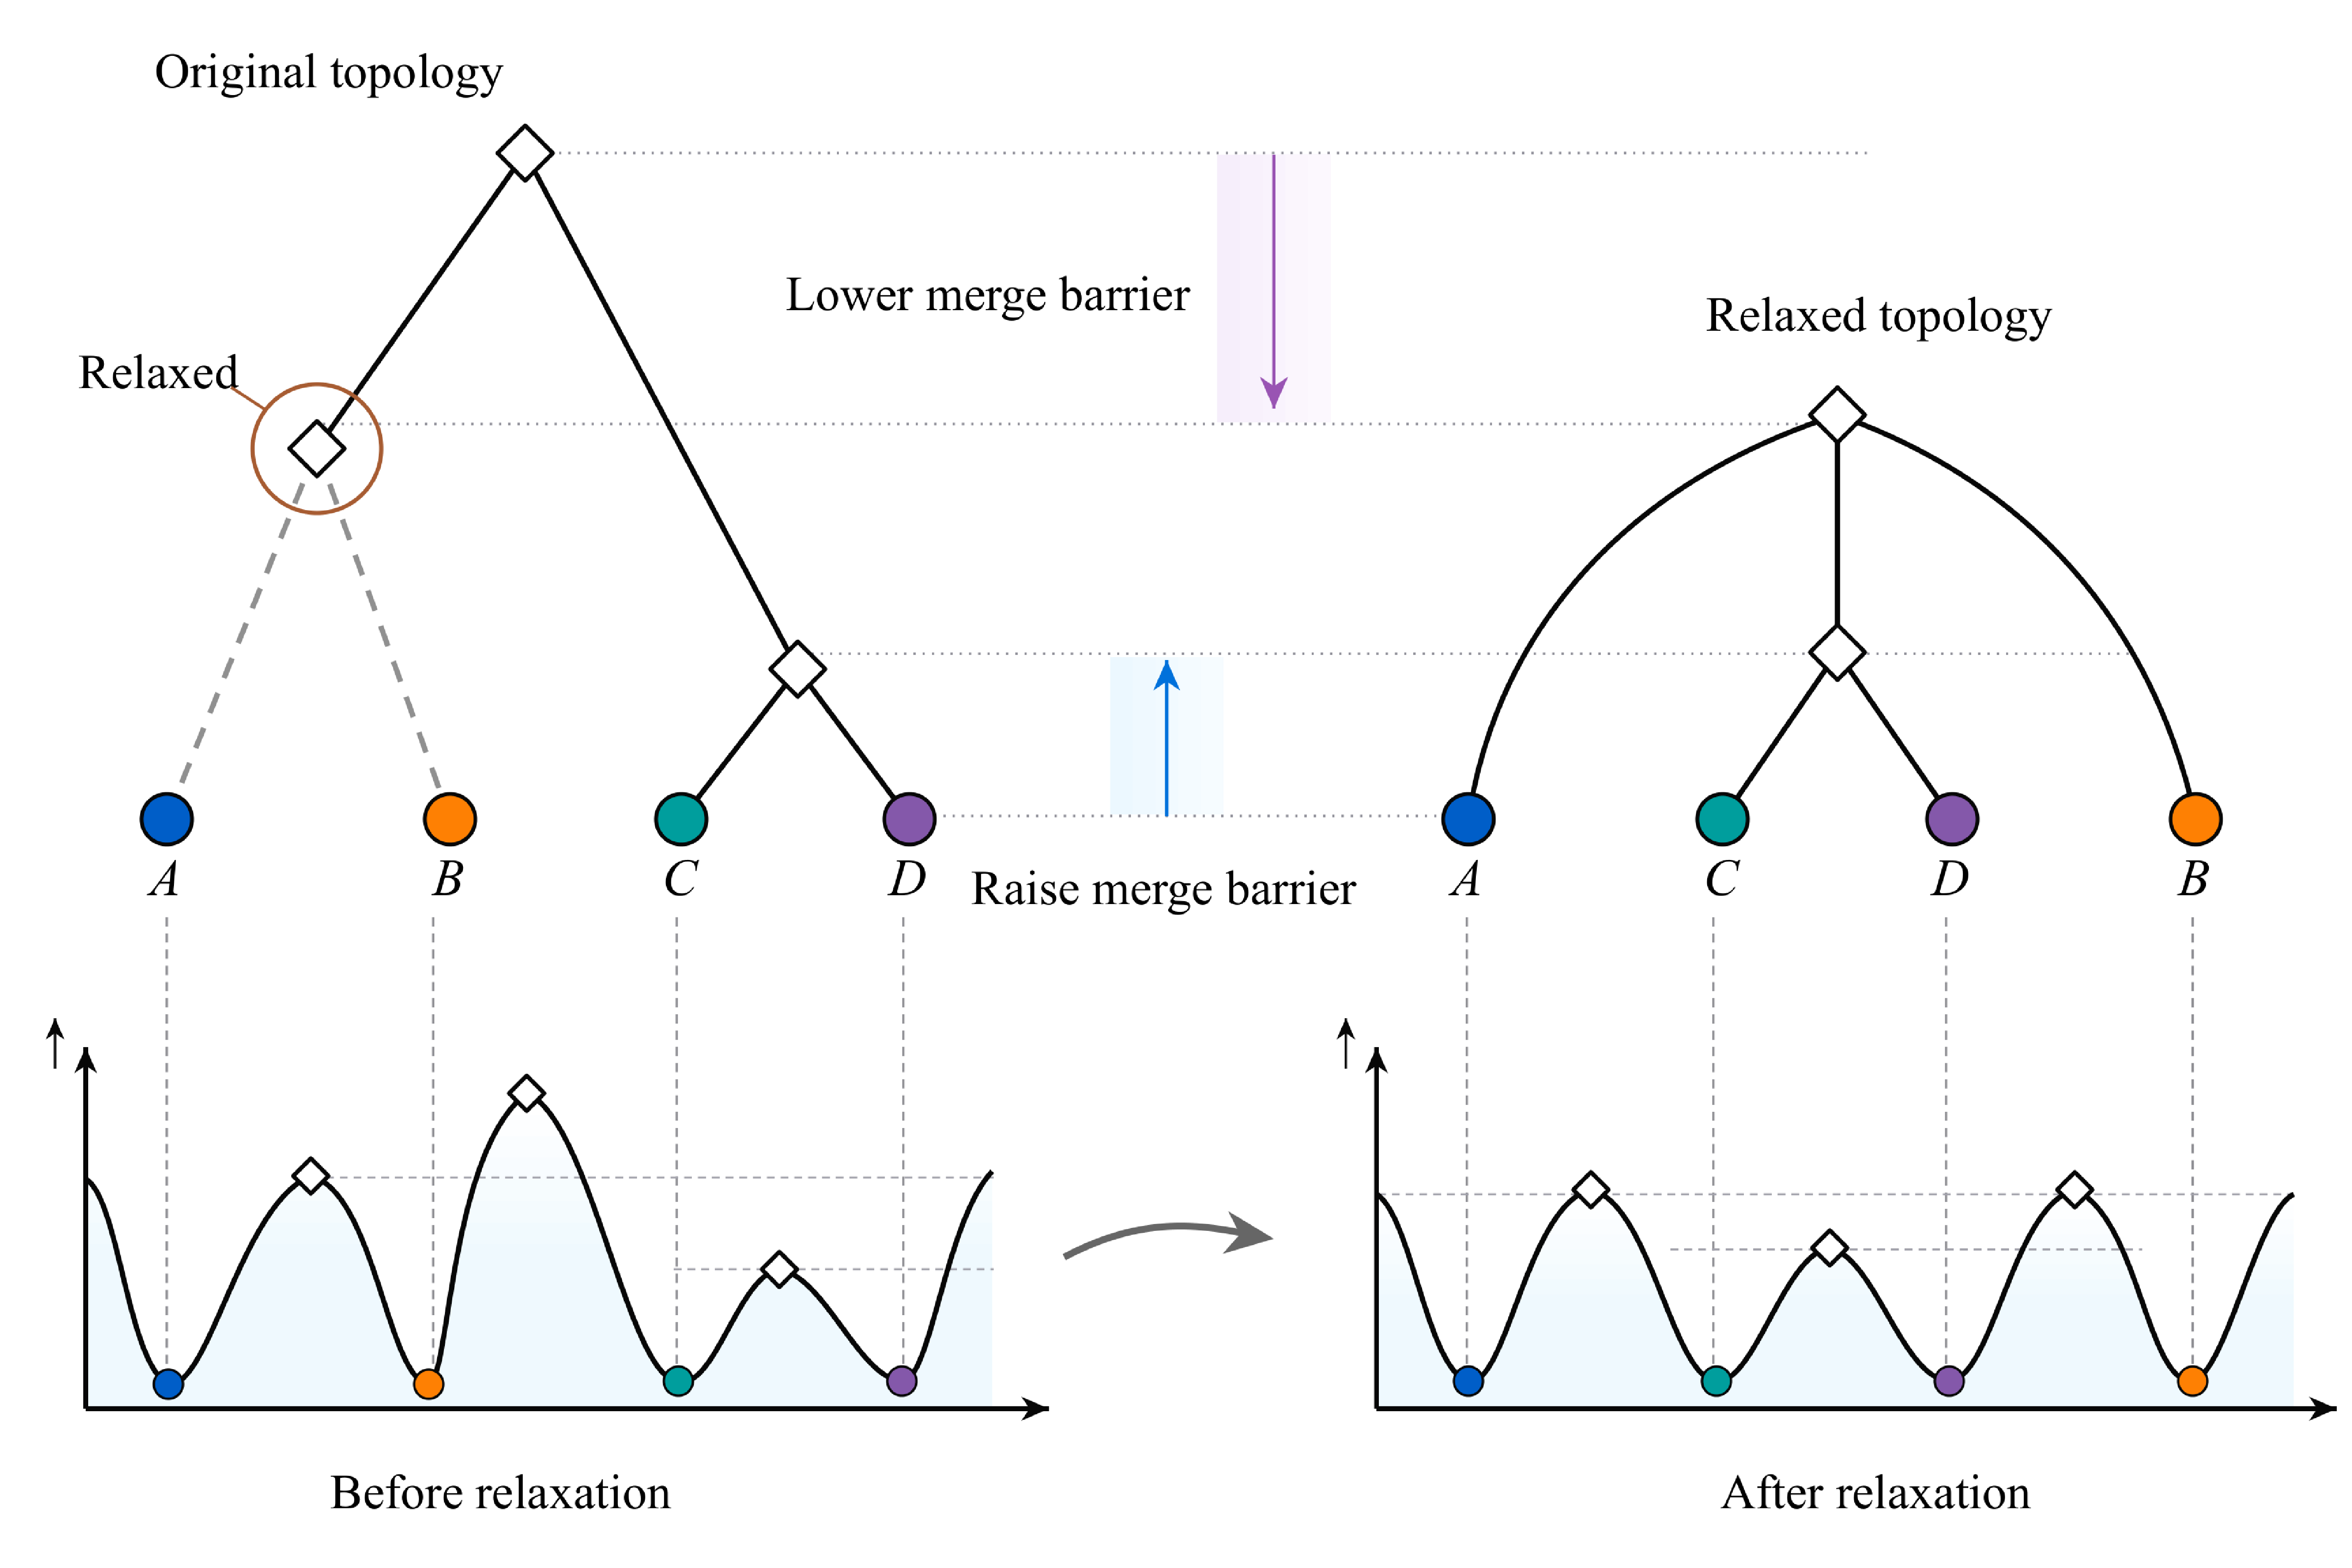
\includegraphics[width=\columnwidth]{figures/anchor_relaxation_open.pdf}
\caption{Selective relaxation releases the $A,B$ block constraint and admits order $A,C,D,B$ while retaining the $C,D$ grouping. The accompanying profiles illustrate changed merge barriers; source-level guides show the hierarchy changes. Heights are schematic, and candidate orders still require evaluation against the original merge matrix.}
\label{fig:selective_relaxation}
\end{figure}
\subsection{Certified Position--Topology Bounds}\label{sec:bounds}
The construction can leave reference displacement even after optimization. The following bounds explain what topology and finite widths make unavoidable: the first answers how much a tree-compatible point order must deviate, the second adds interval packing, and the third asks which restrictions survive a merge-error allowance. They are analytical benchmarks, not three execution stages or search-pruning rules; construction uses the exact fixed-order costs $\tau$ and $\delta^*$. The resulting certificates apply independently of the layout algorithm. Full proofs and computational definitions accompany the paper in Supplementary Material. We suppress $t$ within a frame, use $[v]^+=\max(v,0)$, and take empty maxima as zero.

\subsubsection{Exact-Topology Reference-Order Bound}
For a reduced tree with strictly increasing proper-ancestor levels, exact topology makes every subtree contiguous. Let $[m_X,M_X]$ be the reference hull of the leaves in subtree $X$.
\begin{theorem}[Exact-Topology Position Bound]\label{thm:order}
Every zero-error profile has $\nroe(\pi)\ge\nu^*(T,q)$, where
\begin{equation}\label{eq:nu}
 \nu^*(T,q)=\frac{1}{2L}\max_v\max_{\substack{X,Y\in\mathrm{ch}(v)\\X\ne Y}}
 [\min(M_X-m_Y,M_Y-m_X)]^+.
\end{equation}
Recursive child ordering by reference-hull midpoint attains this point-model order bound in $O(n\log n)$ time.
\end{theorem}
\begin{proof}[Proof sketch]
Sibling blocks must choose one orientation. Their two possible inversion costs are $[M_X-m_Y]^+/2$ and $[M_Y-m_X]^+/2$. Midpoint order chooses the smaller; every inverted leaf pair is separated by sibling blocks at its LCA.
\end{proof}
The maximizing node and sibling pair say where the cost arises, at the merge of two subtrees whose projected ranges overlap, and the value says how much: half the overlap that remains in the cheaper orientation. Midpoint ordering attains the point-order optimum; finite intervals introduce additional constraints, considered next.

\subsubsection{Width-Aware Position Bound}
Finite widths, minimum gaps, anchor slack and canvas capacity add packing costs to the point-order obstruction. For a nonempty leaf set $S$, let $H_i=\rho W_i/2$, $\ell_i=q_i-W_i/2-H_i$, $h_i=q_i+W_i/2+H_i$, and $s_i=W_i+g$. Define two packing summaries:
\begin{equation}\label{eq:packing}
\begin{aligned}
 A(S)&=\max_{a\in S}\left(\ell_a+\sum_{\substack{i\in S\\\ell_i\ge\ell_a}}s_i\right),\\
 B(S)&=\max_{b\in S}\left(\sum_{\substack{i\in S\\h_i\le h_b}}s_i-h_b\right).
\end{aligned}
\end{equation}
The first uses upper reference-endpoint sets and the second lower sets; sorting and cumulative sums evaluate them. For disjoint leaf sets $X,Y$ and the full leaf set $\mathcal{F}$, write
\begin{equation}\label{eq:packingcost}
\begin{aligned}
 \omega(X,Y)&=\tfrac12\min\{A(X)+B(Y),A(Y)+B(X)\}-\tfrac g2,\\
 E_\partial&=\max\{0,B(\mathcal{F})-g,A(\mathcal{F})-g-L\}.
\end{aligned}
\end{equation}
Here $\omega$ takes the cheaper block orientation and $E_\partial$ accounts for both canvas ends. Let $\mathcal{P}_0$ contain every pair of distinct sibling descendant-leaf sets. The certificate is
\begin{equation}\label{eq:bwdef}
 \mathcal{B}_w(T,q,W)=\max\{E_\partial,\max_{(X,Y)\in\mathcal{P}_0}\omega(X,Y)\}.
\end{equation}
The dependence on $g$, $\rho$ and $L$ is through Eqs.~\ref{eq:packing}--\ref{eq:packingcost}; it is suppressed in the certificate's arguments.
\begin{theorem}[Width-Aware Position Bound]\label{thm:width}
For any feasible exact-topology interval layout,
\begin{equation}\label{eq:widthbound}
 \|x-q\|_\infty\ge\tau(\pi)\ge\mathcal{B}_w(T,q,W).
\end{equation}
With zero widths and gaps, $\mathcal{B}_w=L\nu^*(T,q)$.
\end{theorem}
\begin{proof}[Proof sketch]
The first and last anchors of selected leaves must enclose their intervals and intervening gaps, up to the allowed anchor slack. Upper and lower sets in Eq.~\ref{eq:packing} maximize the resulting shortfall against reference separation. Exact topology requires one orientation of every sibling pair; the canvas ends give the two one-sided costs.
\end{proof}
Thus $\mathcal{B}_w$ bounds all exact-topology legal interval orders and need not be attained; $\tau(\pi)$ is the attained minimum for a specified order. These quantities have coordinate units, whereas NROE and $\nu^*$ are normalized by $L$.

\begin{table}[!ht]
\centering
\caption{Planar parameter settings and runtime (seconds): Balanced on the benchmark inputs, a fixed 5\% budget on PM$_{2.5}$.}
\label{tab:anchor-parameters-final}
\footnotesize
\setlength{\tabcolsep}{2pt}
\renewcommand{\arraystretch}{0.95}
\begin{tabular}{@{}lccccc@{}}
\toprule
Parameter & Gaussian & Ring & Wildfires & Storms & PM$_{2.5}$ \\
\midrule
$\varepsilon$ & 1\% & 1\% & 5\% & 10\% & 5\% \\
$N_r$ & 4096 & 196 & 4096 & 4096 & 4096 \\
$s_w$ & 0.00581 & 0.00328 & 0.00053 & 0.01170 & 0.00073 \\
$t_{opt}$ & 0.156 & 0.150 & 3.324 & 2.600 & 199.975 \\
$t_{total}$ & 1.340 & 0.486 & 4.424 & 63.447 & 231.177 \\
\bottomrule
\end{tabular}
\vspace{2pt}
\begin{minipage}{0.94\columnwidth}\footnotesize Weights $(4,1,0.5,0.1)$ and $\rho=0.5$ are fixed. $s_w$ is width per support measure; $N_r$ is raster length. Times are one uncached run on Apple M4: optimization and full pipeline, respectively.\end{minipage}
\end{table}

\definecolor{pubgray}{gray}{0.45}
\begin{table*}[t]
\centering
\caption{Five-dataset comparison. Bold/underline mark the best/second distinct local measurements per dataset; ties share emphasis. Curves use fixed default orientations.}
\label{tab:quantitative-final}
\footnotesize
\setlength{\tabcolsep}{1.5pt}
\renewcommand{\arraystretch}{0.85}
\begin{tabular*}{\textwidth}{@{\extracolsep{\fill}}l*{12}{c}lccc@{}}
\toprule
\multirow{2}{*}{Dataset} & \multicolumn{3}{c}{Hilbert} & \multicolumn{3}{c}{Morton} & \multicolumn{3}{c}{TMTM} & \multicolumn{3}{c}{ST-MTM} & \multicolumn{4}{c}{AnchorMTM (ours)} \\
\cmidrule(lr){2-4}\cmidrule(lr){5-7}\cmidrule(lr){8-10}\cmidrule(lr){11-13}\cmidrule(lr){14-17}
 & SNS$\downarrow$ & TW$\uparrow$ & NPE$\downarrow$ & SNS$\downarrow$ & TW$\uparrow$ & NPE$\downarrow$ & SNS$\downarrow$ & TW$\uparrow$ & NPE$\downarrow$ & SNS$\downarrow$ & TW$\uparrow$ & NPE$\downarrow$ & Mode & SNS$\downarrow$ & TW$\uparrow$ & NPE$\downarrow$ \\
\midrule
\multirow{2}{*}{Gaussian} & \multirow{2}{*}{$0.1117$} & \multirow{2}{*}{$0.6719$} & \multirow{2}{*}{$0.7557$} & \multirow{2}{*}{$\underline{0.0393}$} & \multirow{2}{*}{$\underline{0.8333}$} & \multirow{2}{*}{$0.7359$} & \multirow{2}{*}{\textcolor{pubgray}{$0.2500^\dagger$}} & \multirow{2}{*}{\textcolor{pubgray}{$0.7700^\dagger$}} & \multirow{2}{*}{$\underline{0.1118}$} & \multirow{2}{*}{\textcolor{pubgray}{$0.0600^\dagger$}} & \multirow{2}{*}{\textcolor{pubgray}{$1.0000^\dagger$}} & \multirow{2}{*}{$0.1154$} & Exact & $\mathbf{0.0353}$ & $\mathbf{0.9323}$ & $\mathbf{0.0089}$ \\
 &  &  &  &  &  &  &  &  &  &  &  &  & Balanced & $\mathbf{0.0353}$ & $\mathbf{0.9323}$ & $\mathbf{0.0089}$ \\
\multirow{2}{*}{Ring} & \multirow{2}{*}{$\mathbf{0.1252}$} & \multirow{2}{*}{$\mathbf{0.9048}$} & \multirow{2}{*}{$0.5941$} & \multirow{2}{*}{$0.1489$} & \multirow{2}{*}{$0.7619$} & \multirow{2}{*}{$0.6033$} & \multirow{2}{*}{\textcolor{pubgray}{$0.2800^\dagger$}} & \multirow{2}{*}{\textcolor{pubgray}{$0.6800^\dagger$}} & \multirow{2}{*}{$0.1756$} & \multirow{2}{*}{\textcolor{pubgray}{$0.2100^\dagger$}} & \multirow{2}{*}{\textcolor{pubgray}{$0.8800^\dagger$}} & \multirow{2}{*}{$0.2463$} & Exact & $0.1485$ & $\underline{0.8571}$ & $\underline{0.0471}$ \\
 &  &  &  &  &  &  &  &  &  &  &  &  & Balanced & $\underline{0.1334}$ & $\underline{0.8571}$ & $\mathbf{0.0395}$ \\
\multirow{2}{*}{Wildfires} & \multirow{2}{*}{$0.1883$} & \multirow{2}{*}{$0.8303$} & \multirow{2}{*}{$0.3641$} & \multirow{2}{*}{$0.1304$} & \multirow{2}{*}{$0.8758$} & \multirow{2}{*}{$0.1560$} & \multirow{2}{*}{\textcolor{pubgray}{$0.4400^\dagger$}} & \multirow{2}{*}{\textcolor{pubgray}{$0.8800^\dagger$}} & \multirow{2}{*}{$0.2280$} & \multirow{2}{*}{\textcolor{pubgray}{$0.2400^\dagger$}} & \multirow{2}{*}{\textcolor{pubgray}{$0.9100^\dagger$}} & \multirow{2}{*}{$0.3180$} & Exact & $\mathbf{0.0426}$ & $\mathbf{0.9136}$ & $\underline{0.0131}$ \\
 &  &  &  &  &  &  &  &  &  &  &  &  & Balanced & $\underline{0.0447}$ & $\underline{0.8989}$ & $\mathbf{0.0116}$ \\
\multirow{2}{*}{Storms} & \multirow{2}{*}{$0.1290$} & \multirow{2}{*}{$0.7403$} & \multirow{2}{*}{$0.3705$} & \multirow{2}{*}{$0.1180$} & \multirow{2}{*}{$0.7251$} & \multirow{2}{*}{$0.3468$} & \multirow{2}{*}{\textcolor{pubgray}{$0.3400^\dagger$}} & \multirow{2}{*}{\textcolor{pubgray}{$0.7100^\dagger$}} & \multirow{2}{*}{$0.5753$} & \multirow{2}{*}{\textcolor{pubgray}{$0.2100^\dagger$}} & \multirow{2}{*}{\textcolor{pubgray}{$0.9400^\dagger$}} & \multirow{2}{*}{$0.4579$} & Exact & $\underline{0.0790}$ & $\underline{0.8463}$ & $\underline{0.0399}$ \\
 &  &  &  &  &  &  &  &  &  &  &  &  & Balanced & $\mathbf{0.0743}$ & $\mathbf{0.8766}$ & $\mathbf{0.0140}$ \\
\multirow{2}{*}{PM$_{2.5}$} & \multirow{2}{*}{$0.2386$} & \multirow{2}{*}{$\mathbf{0.8887}$} & \multirow{2}{*}{$0.8090$} & \multirow{2}{*}{$\underline{0.1760}$} & \multirow{2}{*}{$\underline{0.8277}$} & \multirow{2}{*}{$0.8823$} & \multirow{2}{*}{$0.3018$} & \multirow{2}{*}{$0.7781$} & \multirow{2}{*}{$0.5241$} & \multirow{2}{*}{$0.1897$} & \multirow{2}{*}{$0.8224$} & \multirow{2}{*}{$0.5577$} & Exact & $0.1964$ & $0.7884$ & $\underline{0.1390}$ \\
 &  &  &  &  &  &  &  &  &  &  &  &  & 5\% & $\mathbf{0.1636}$ & $0.7657$ & $\mathbf{0.0468}$ \\
\bottomrule
\end{tabular*}
\vspace{2pt}
\begin{minipage}{\textwidth}\footnotesize $^\dagger$Grey: published TMTM/ST-MTM Temporal SNS/TW on the four benchmark inputs (ST-MTM Table~1, authors' inputs), shown for reference and excluded from emphasis; all other entries, including every PM$_{2.5}$ value, are local measurements on the same inputs. Author inputs and coverage are unconfirmed. Local TW coverage (Gaussian/Ring/Wildfires/Storms/PM$_{2.5}$) is 64/64, 1/40, 4/32, 11/744, 744/744; ineligible frames are omitted. Published TW has two-decimal precision. Mode applies only to AnchorMTM; PM$_{2.5}$ uses a fixed 5\% budget, not a selected Balanced budget.\end{minipage}
\end{table*}

\subsubsection{Bounded-Topology Position Bound}
A merge-level allowance can release some contiguous blocks, but still limits interleaving. If leaf $k$ lies between descendants $i,j$ of node $u$, interval containment gives $V_{ik}^{\psi}\le V_{ij}^{\psi}$, hence $V_{ik}\le h(u)+2\eta$. Define $A_\eta(u)$ as the highest ancestor, including $u$, with $h(A_\eta(u))-h(u)\le2\eta$. This uses the accumulated ancestor-height difference in scalar units, on the reduced equal-level tree with the fixed labels of Eq.~\ref{eq:dtop}.

Let $\mathcal{P}_\eta$ consist of two types of leaf-set pairs: $(\mathcal{D}(u),\{k\})$ for every internal node $u$ and leaf $k\notin\mathcal{D}(A_\eta(u))$; and $(\mathcal{D}(u),\mathcal{D}(w))$ for internal nodes $u,w$ satisfying
\begin{equation}\label{eq:separatedpairs}
\begin{aligned}
 \mathcal{D}(w)\cap\mathcal{D}(A_\eta(u))&=\varnothing,\\
 \mathcal{D}(u)\cap\mathcal{D}(A_\eta(w))&=\varnothing.
\end{aligned}
\end{equation}
For any nonempty leaf set $X$, use its reference hull $[m_X,M_X]$ and define $\kappa(X,Y)=[\min(M_X-m_Y,M_Y-m_X)]^+/(2L)$. The two certificates are
\begin{equation}\label{eq:chaindef}
\begin{aligned}
 C_\eta(T,q)&=\max_{(X,Y)\in\mathcal{P}_\eta}\kappa(X,Y),\\
 C_{w,\eta}(T,q,W)&=\max\{E_\partial,\max_{(X,Y)\in\mathcal{P}_\eta}\omega(X,Y)\}.
\end{aligned}
\end{equation}
\begin{theorem}[Bounded-Topology Position Bound]\label{thm:chain}
In a profile with $\dtop\le\eta$, no leaf outside $\mathcal{D}(A_\eta(u))$ can lie between two leaves of $u$. Every pair in $\mathcal{P}_\eta$ lies wholly in one block orientation or the other. Consequently,
\begin{equation}\label{eq:chainbounds}
 \nroe(\pi)\ge C_\eta(T,q),\qquad
 \tau(\pi)\ge C_{w,\eta}(T,q,W),
\end{equation}
with the second inequality applying to the interval model.
\end{theorem}
The separation principle excludes interleaving for each eligible pair; the two possible orientations then yield $\kappa$ and $\omega$. Thus $C_\eta$ bounds normalized reference-order error, while $C_{w,\eta}$ includes finite-width and boundary costs in coordinate units. Flattening every parent gap of at most $2\eta$ gives a second valid certificate; neither dominates, since flattening also separates single-leaf pairs that $\mathcal{P}_\eta$ omits, and we report the larger. The pair set also says what releases a conflict: a subtree may interleave with its sibling once $2\eta$ reaches the gap between its own merge level and its parent's, so conflicts at deep merges stay expensive.

The allowance concerns the displayed hierarchy; the source field and feature identities stay fixed. A larger feasible set need not improve every feature or every heuristic result. These bounds are reported as benchmarks for unavoidable error; ranking and continuous acceptance use the exact fixed-order evaluations in Section~\ref{sec:construction}. Continuous feasibility does not certify the full rendered raster.

